\documentclass[10pt,a4paper,onecolumn]{article}
\usepackage[T1]{fontenc}
\usepackage[utf8]{inputenc}
\usepackage[brazilian]{babel}
\usepackage[left=1.5cm,right=1.5cm,top=2.5cm,bottom=2cm]{geometry}
\usepackage[pdftex]{xcolor,graphicx}
\usepackage{amsmath}
\usepackage{amsfonts}
\usepackage{amssymb}
\usepackage{amsthm}
\usepackage{ae}
\usepackage{indentfirst}
\usepackage{multicol}
\usepackage{listings}

\renewcommand{\sp}{{\footnotesize \#}}

\definecolor{codegreen}{rgb}{0,0.6,0}
\definecolor{codegray}{rgb}{0.5,0.5,0.5}
\definecolor{codepurple}{rgb}{0.58,0,0.82}
\definecolor{backcolour}{rgb}{0.95,0.95,0.92}

\lstdefinestyle{mystyle}{
	backgroundcolor=\color{backcolour},   
	%keywordstyle=\color{magenta},
	numberstyle=\tiny\color{black},
	stringstyle=\color{codegreen},
	%basicstyle=\ttfamily\footnotesize,
	breakatwhitespace=false,         
	%breaklines=true,                 
    %captionpos=b,                    
	keepspaces=true,                 
	numbers=left,                    
	%numbersep=5pt,                  
	showspaces=false,                
	showstringspaces=false,
	%showtabs=false,                  
	tabsize=2,	
	otherkeywords={with},
	morekeywords=[2]{1, 2, 3, 4, 5, 6, 7, 8, 9, 0},
	keywordstyle=[2]{\color[HTML]{ff0bff}},
	%keywordstyle=\color{blue}\bfseries,
	%stringstyle=\color{red},
	basicstyle=\ttfamily,
	tabsize=4,    
	columns=fixed,
	extendedchars=false,
	breaklines=true,
	keywordstyle=\bfseries\color[HTML]{d52a2a}, 
	keywordstyle=[2]\color[HTML]{008a8c},
	commentstyle=\color[HTML]{0000a0},
	%stringstyle=\color[HTML]{ff0bff},
	%numberstyle=\color[HTML]{ff0bff},
	commentstyle=\color{blue},
	literate={”“}{``''}1
}
 
\lstset{style=mystyle}


\newcommand{\Ll}{L^{2}\left(\Rn\right)}
\renewcommand{\qedsymbol}{$\blacksquare$}
%\renewcommand{\chaptername}{} 

\pagestyle{headings}

\theoremstyle{definition}
\newtheorem{definition}{Definition}[section] 
\newtheorem{proposition}[definition]{Proposition}
\newtheorem{theorem}[definition]{Theorem}
\newtheorem{lemma}[definition]{Lemma}
\newtheorem{corollary}[definition]{Corollary}
\newtheorem{scholium}[definition]{Scholium}

\theoremstyle{remark}
\newtheorem{remark}{Remark}[section]
\newtheorem{example}[remark]{Example}

\newcommand{\tamanho}{\footnotesize}
\newcommand{\tamanhocaption}{\footnotesize}

\begin{document}
\title{\huge \textbf{Distribuição de \emph{tags} de POS em Cícero e sua variação no tempo e segundo o gênero} \\ \Large FLL 5133 -- 2021}
\author{\large Victor Chabu} 
\date{}
\maketitle

\section{Introdução}
No EP 7 desenvolvido neste semestre, avaliou-se a possibilidade de caracterizar a autoria de um texto por meio de marcadores linguísticos referentes a partes do discurso (POS). A hipótese de base era que um autor, escrevendo em um certo gênero, tende a produzir sentenças cujas partes do discurso obedeçam a uma distribuição de probabilidades estável. Embora não seja absurdo pensar que alguns marcadores de POS sejam mais relevantes que outros para esse tipo de análise, e mesmo que um ou outro possa ser por si só determinante, o objetivo ali foi estudá-los individualmente, mas sim em conjunto. 

Tomamos $\mu_1,\dots,\mu_n$ como médias por sentença da densidade\footnote{A densidade aqui calculada como o número total de ocorrências do marcador de POS em uma sentença dividido pelo tamanho dessa sentença medido em \emph{tokens}.} dos marcadores $1,\dots,n$ produzidas por dado autor escrevendo em um determinado gênero, distribuídas com variâncias $\sigma_1^2,\dots,\sigma_n^2$; avaliamos quantidade:
\begin{equation}\label{eq:chi}
	\chi^2 = \sum_{i = 1}^{n} \left( \frac{x_i-\mu_i}{\sigma_i} \right)^2,
\end{equation}
em que $x_i$ representam as médias de marcadores POS por sentença medidas em um texto cuja autoria se queira determinar.

Se cada $x_i$ for uma variável aleatória gaussiana de média $\mu_i$ e variância $\sigma_i^2$ independente de $x_j$, $j \neq i$, então $\chi^2$ deverá ser uma variável aleatória distribuída como um qui-quadrado de média $n$ e variância $2n$, e poderemos aplicar um teste de confiança de qui-quadrado padrão para determinar se o texto em análise é compatível com a produção de determinado autor.

Essa abordagem apresenta algumas dificuldades importantes que precisaram ser dirimidas. 
\begin{itemize}
	\item A primeira delas é que as variáveis $x_i$ não podem ser perfeitamente gaussianas, já que, por serem contagens, temos sempre $x_i \geqslant 0$; além disso, temos desvios padrões relativos muitas vezes superiores a 1 (chegamos a ter $\frac{\sigma}{\mu} \sim 40$ para alguns marcadores). Ora, uma variável positiva com desvio padrão maior que a média não pode ser nem mesmo simétrica, muito menos gaussiana.
	\item Para os textos utilizados como \emph{corpora} naquele EP (\emph{O Guarani} de José de Alencar, \emph{O Abolicionismo} de Luís Gama, e \emph{Dom Casmurro}, de Machado de Assis) houve correlações entre $x_i$ e $x_j$, $i \neq j$, que chegavam à ordem de 40\%, o que descaracterizaria a quantidade $\chi^2$ em \eqref{eq:chi} como um qui-quadrado mesmo que tivéssemos variáveis $x_1,\dots,x_n$ perfeitamente gaussianas.
	\item Não dispúnhamos de nenhum modelo que fornecesse valores teóricos $\mu_i$ e $\sigma_i$ para cada autor, devendo esses ser substituídos por estimadores $m_i$ e $s_i$ calculados a partir de dados obtidos em \emph{corpora} disponíveis para os diversos autores.
	
	 Com relação à média, não há problema, já que podemos absorver a flutuação estatística de $m_i$ naquela de $x_i$. Com efeito, estimando $\mu_i$ em uma amostra com $N$ dados, tomamos $m_i = \mu_i + \varepsilon_i$, em que $\varepsilon_i$ é uma variável aleatória de média $0$, e obtemos:
	$$x_i - m_i = (x_i - \varepsilon_i) - \mu_i = y_i - \mu_i,$$
	em que $y_i$ é uma variável aleatória com média $\mu_i$ e variância:
	$$\sigma^2_{y_i} = \sigma_i^2 + \frac{\sigma_i^2}{N},$$
	em que $\sigma^2_{m_i} = \frac{\sigma_i^2}{N}$ é simplesmente a variância do estimador $m_i$ da média para $N$ dados. 
	
	O mesmo não pode ser feito de maneira direta com relação à variância. Na realidade, se uma variável do tipo 
	$$g \sim \frac{x-\mu}{\sigma}$$
	é gaussiana, sabemos que a variável correspondente substituindo o desvio padrão por seu estimador $s$,
	$$t \sim \frac{x-\mu}{s},$$
	será distribuída segundo a função $t$ de Student. Qualitativamente, o $t$ Student assemelha-se à curva normal, exceto que ``mais larga'', refletindo o fato de que a flutuação do estimador $s$ insere na variável $t$ uma incerteza adicional que $g$ não tinha.
	
	Ora, aqui não é claro nem sequer se as variáveis $x_i$ podem ser adequadamente aproximadas por gaussianas, de modo que a diferença entre $t$ e $g$ será ignorada.
	
	Como resultado, calculamos experimentalmente a variável:
	\begin{equation}\label{eq:meuqui}
		\chi^2 = \sum_{i = 1}^n \frac{(x_i-m_i)^2}{s_i^2\left(1 + \frac{1}{N}\right)}.
	\end{equation}
\end{itemize}

Assim, para a variável aleatória $\chi^2$ em \eqref{eq:meuqui}, os valores $m_i$ e $s_i$ foram obtidos dos \emph{corpora} disponíveis para cada autor, e $x_i$ foram dados medidos no texto cuja autoria se queria identificar, no caso, \emph{Ubirajara}, de José de Alencar.   

A fim de dar conta dos problemas levantados acima, discutiu-se naquele trabalho que o melhor procedimento seria calcular as densidades de marcadores de POS a partir de grupos de médias 50 sentenças aleatoriamente selecionadas de cada texto, restringindo-nos apenas àqueles marcadores cujas distribuições mais se assemelhassem a gaussianas, e que apresentassem menores correlações entre si\footnote{Correlação não implica dependência, mas o contrário sim, de modo que apenas considerar variáveis pouco correlacionadas é uma forma de certificar-se de que sejam também independentes.}, de modo que, das 23 \emph{tags} disponíveis para língua portuguesa, utilizamos apenas  
\begin{verbatim}
	ADJ, PROPN, ADP, PUNCT, ADV, SCONJ, AUX, NOUN, CCONJ, VERB, DET, PRON,
\end{verbatim} 
além da variável \texttt{Tam} referente ao tamanho médio das sentenças, em \emph{tokens}.

A partir de tal procedimento, calculamos o valor da variável $\chi^2$ definida em \eqref{eq:meuqui}, seu desvio padrão, e os correspondentes valores para o $\chi^2$ reduzido, considerando os dados obtidos de \emph{Ubirajara} e as estatísticas referentes às distribuições nos diversos textos do \emph{corpus}, chegando aos seguintes resultados:

\begin{verbatim}
	Guarani.txt       | X2 = 26.37 +- 5.10, X2_redux = 2.03 +- 0.39, gdl = 13
	DomCasmurro.txt   | X2 = 124.81 +- 5.10, X2_redux = 9.60 +- 0.39, gdl = 13
	Abolicionismo.txt | X2 = 75.24 +- 5.10, X2_redux = 5.79 +- 0.39, gdl = 13
\end{verbatim}
Repetindo o cálculo diversas vezes para observar a variação desses valores com as diferentes seleções aleatórias de 50 sentenças sobre as quais calculamos das densidades das \emph{tags}, obtivemos valores consistentes:

\begin{verbatim}
	Guarani.txt       | X2 = 25.36 +- 5.10, X2_redux = 1.95 +- 0.39, gdl = 13
	DomCasmurro.txt   | X2 = 91.87 +- 5.10, X2_redux = 7.07 +- 0.39, gdl = 13
	Abolicionismo.txt | X2 = 94.91 +- 5.10, X2_redux = 7.30 +- 0.39, gdl = 13
\end{verbatim}

\begin{verbatim}
	Guarani.txt       | X2 = 25.88 +- 5.10, X2_redux = 1.99 +- 0.39, gdl = 13
	DomCasmurro.txt   | X2 = 101.48 +- 5.10, X2_redux = 7.81 +- 0.39, gdl = 13
	Abolicionismo.txt | X2 = 119.15 +- 5.10, X2_redux = 9.17 +- 0.39, gdl = 13
\end{verbatim}

\begin{verbatim}
	Guarani.txt       | X2 = 30.65 +- 5.10, X2_redux = 2.36 +- 0.39, gdl = 13
	DomCasmurro.txt   | X2 = 107.35 +- 5.10, X2_redux = 8.26 +- 0.39, gdl = 13
	Abolicionismo.txt | X2 = 77.51 +- 5.10, X2_redux = 5.96 +- 0.39, gdl = 13
\end{verbatim}

Como se pôde ver, em qualquer uma das 4 iterações do programa houve uma clara diferença no valor de $\chi^2$ obtido para José de Alencar ou para os outros autores, o que \underline{parece compatível} com o fato de que, efetivamente, \emph{Ubirajara} é um romance de José de Alencar em sua fase indianista, assim como \emph{O Guarani}. Entretanto, tais resultados suscitaram diversos questionamentos sobre a compatibilidade das distribuições de \emph{tags} de POS em textos de um mesmo autor em períodos diferentes de sua produção, ou quando ele escreve segundo gêneros literários reconhecidamente distintos, ao mesmo tempo que se pergunta se algumas das \emph{tags} obedeceriam a distribuições mais típicas de cada autor, portanto mais determinantes de autoria.

\break

À guisa de resposta, precisaríamos estudar a distribuição de \emph{tags} de POS na obra de diversos autores cuja produção se estenda ao longo do tempo e que também se notabilizem pela variedade de temas e gêneros. Um autor com essas características é Marco Túlio Cícero, cuja trabalho estende-se por 40 anos, abrange os mais diversos assuntos, e assume formas bastante distintas, com um amplo conjunto de discursos políticos e judiciais (aqui agrupados no gênero \texttt{oratoria}), de correspondência com amigos e familiares (gênero \texttt{epistola}), e uma importante obra filosófica (gênero \texttt{filosofia}) geralmente no formato de diálogo. Neste artigo, analisaremos a distribuição de POS no \emph{corpus} ciceroniano, a fim de estabelecer uma metodologia que possibilite responder às questões do parágrafo anterior.    

Além disso, proporemos algumas modificações serão necessárias nos procedimentos empregados no EP 7, uma vez que ali o \emph{corpus} de cada autor era um conjunto de grupos de 50 sentenças extraídas de um mesmo texto, e na nova análise precisaremos lidar com diversos textos agrupados por gênero ou por período; em outras palavras, enquanto ali testávamos a compatibilidade da distribuição de \emph{tags} de um texto com a do outro, aqui precisaremos testar a distribuição de \emph{tags} em um texto com um conjunto de outros, que não necessariamente possuem as mesmas distribuições entre si. Não é claro, por exemplo, como os resultados seriam afetados se concatenássemos os diversos textos de um gênero, e do texto total resultante fizéssemos as seleções de 50 sentenças calculando daí estatísticas para uma \underline{distribuição única por gênero}, ou se tomássemos individualmente cada texto e para ele calculássemos as estatísticas para cada um, e delas as estatísticas para uma \underline{distribuição de distribuições por gênero}. Essa dúvida metodológica reflete uma questão de fundo muito relevante, que é saber se, dentro de um gênero, em um período determinado, as variações de estilo devem-se sobretudo às idiossincrasias do autor, ou às condições tópicas de produção de cada texto.

Uma análise qualitativa de Cícero faz-nos tender fortemente à segunda hipótese. É dele o único caso conhecido de um discurso antigo que sobreviveu até a atualidade em duas versões completas, uma dirigida ao Senado romano e outra à assembleia popular. Nesse discurso, em que Cícero ataca Marco Antônio e defende a posição de Otaviano na guerra civil, nota-se que na elocução senatorial os períodos tendem a ser mais longos, mais complexos, com mais níveis de subordinação e inversões sintáticas, e o próprio texto é mais longo que sua versão concional, mais curta e direta. Não obstante, pode ser que algumas POS variem de forma essencialmente idiossincrática (talvez \texttt{ADV} ou \texttt{ADJ}?), enquanto que outras (como a prevalência de \texttt{SCONJ} para o caso de sucessivas subordinações) realmente dependa mais do contexto e do público alvo.

Assim, neste estudo preliminar consideraremos que cada texto é uma realização de uma variável aleatória valorada em outra distribuição, ou seja, consideraremos que dentro de cada gênero há um intervalo de valores médios e desvios padrões que as distribuições de \emph{tags} de POS podem com alguma probabilidade assumir. Dessa maneira, o $i$-ésimo texto do gênero $g$ terá uma média de densidade da \emph{tag} de POS $p$ que chamaremos de $m_i^p$, calculada sobre 48 sentenças\footnote{Essa quantidade foi determinada por tentativa e erro, segundo se constatou que ao agrupar 48 sentenças aleatórias produziam-se variáveis com menores correlações e desvios padrões, resultando em um número maior de \emph{tags} utilizáveis para a análise de $\chi^2$.} aleatoriamente selecionadas do texto, e respectivo desvio padrão da média $\sigma_{m^p_i}$; a média da densidade da \emph{tag} $p$ para o gênero $g$ poderá ser estimada, portanto, por:   
$$m_g^p = \sum_i \frac{m_i^p}{\sigma^2_{m_i^p}} \left( \sum_{i} \frac{1}{\sigma^2_{m_i^p}} \right)^{-1},$$
sendo a variância dessa média estimada por:
$$\frac{1}{\sigma_{m_g^p}^2} = \sum_{i} \frac{1}{\sigma^2_{m_i^p}};$$
a variância simples dessa distribuição relativa às $M$ distribuições de $p$ no gênero $g$ (uma para cada texto) será estimada pela estatística:
$$\left(s^p_g\right)^2 = \frac{1}{M-1} \sum_i \left(m^p_i-m^p_g\right)^2.$$
Finalmente, avaliaremos a compatibilidade de um texto $x$ -- o qual possui densidades médias $x^p$ das \emph{tags} de POS e variâncias da média $\sigma_{x^p}^2$ -- com relação ao gênero $g$ por meio da quantidade: 
\begin{equation}\label{eq:chi_definitivo}
\chi^2_g(x) = \sum_p \frac{\left(x^p - m_g^p\right)^2}{\left(s^p_g\right)^2 + \sigma_{m_g^p}^2 + \sigma_{x^p}^2},
\end{equation}
a qual, espera-se, deve se comportar como um qui-quadrado com $N-1$ graus de liberdade, sendo $N$ a quantidade de \emph{tags} empregada na soma em \eqref{eq:chi_definitivo}.

\medskip

Os textos de Cícero utilizados neste trabalho foram obtidos a partir do repositório \emph{The Latin Library}\footnote{Disponível em \texttt{https://www.thelatinlibrary.com}, acessado em 20/12/2021.}, e a \emph{tokenização} e a análise de POS feitas por meio da biblioteca \texttt{CLTK} disponível em \textsc{Python}\footnote{\texttt{http://cltk.org}, acessado em 20/12/2021}. Todos os arquivos produzidos ao longo do trabalho (códigos, bancos de dados, gráficos, arquivos \texttt{csv}, etc.) estarão disponíveis até 31/01/2022 no endereço \texttt{https://github.com/vbchabu/fll5133\_trabalho\_final}.

\section{Metodologia}\label{sec:metodologia}
A metodologia utilizada seguiu a risca a prescrição da fórmula \eqref{eq:chi_definitivo} para o cálculo do $\chi^2$; mesmo assim, alguns pontos merecem ser comentados referentes ao processamento dos textos latinos anterior às análises estatísticas e à escolha das \emph{tags} a empregar.

\begin{itemize}
	\item A ferramenta de análise de POS do \texttt{CLTK} provou-se pouco confiável, apresentando uma tendência a classificar uma série de elementos como \texttt{NOUN}, ainda que não o fossem, ou ainda que fossem nomes próprios, portanto \texttt{PROPN}. Ela se mostrou frágil frente às grandes variações sintáticas permitidas pela língua latina. Na frase \emph{quod me amas bene scio} (lt. \emph{que me amas, bem sei}), \emph{quod} foi classificado como um pronome \texttt{PRON}, ainda que em realidade seja uma conjunção subordinante \texttt{SCONJ} (o \emph{que} da versão em português); por outro lado, invertendo a ordem do período para \emph{bene scio quod me amas} (lt. \emph{bem sei que me amas}), o \emph{quod} foi corretamente classificado como \texttt{SCONJ}. Da mesma maneira, prenomes, que em latim aparecem abreviados, \emph{I.} (Júlio), \emph{Gn.} (Gnaio), \emph{M.} (Marco), \emph{C.} (Caio), etc., foram classificados de maneiras nem sempre difíceis de explicar, oscilando entre numeral, advérbio, nome e nome próprio, ainda que o \emph{tokenizador} do \texttt{CLTK} quase sempre (mas não sempre) tenha entendido o ponto como uma abreviação, e não como ponto final.   
\end{itemize}

Por esse motivo, já na fase de pré-processamento do texto resolvemos as siglas de prenomes removendo o ponto da abreviatura (de modo a que o \emph{tokenizador} não quebrasse uma sentença única em duas). Quanto aos problemas da classificação de POS, não houve o que fazer, dado o tempo e o escopo do trabalho. Mesmo assim, alguma classificação foi produzida, portanto podemos dizer que essa classificação é a que ocorre segundo uma variável aleatória. Tal abordagem de ``caixa-preta'', em que estudamos a distribuição de \emph{tags} que o algoritmo produz, sem que saibamos ao certo por quais razões, permitiu levar o trabalho a cabo e gerou resultados instigantes (ver Seção \ref{sec:discussao}), ainda que às expensas do significado linguístico das variáveis aleatórias estudadas. Uma das perdas sofridas, é que não podemos afirmar que os discursos senatoriais de Cícero possuam períodos compostos mais ou menos complicados que os concionais com base nas médias da \emph{tag} \texttt{SCONJ}, pois vimos que o \texttt{CLTK} não hesita em classificar conjunções subordinantes como pronomes quando a subordinada aparece, como é frequente em Cícero, antes da oração principal.

\begin{itemize}
	\item Assim como no EP 7, apareceram correlações importantes entre as variáveis aleatórias, e muitas delas exibiram desvios padrões altos demais para que pudessem ser aproximadas por gaussianas. O procedimento de concatenar certa quantidade de sentenças aleatoriamente escolhidas do texto (aqui, 48) foi o suficiente para amenizar o problema na maioria dos casos, mas algumas das amostras de texto, até mesmo por seu estado excessivamente fragmentário, continuaram problemáticas. Foi necessário excluir da análise algumas \emph{tags} e alguns dos textos existentes no \emph{corpus} ciceroniano, porém, com uma quantidade de amostras muito maior que no EP 7, foi necessário automatizar a tarefa de seleção utilizando o algoritmo \texttt{tagselect} (ver Apêndice \ref{ap:tagselect}). 
\end{itemize}
	
Segundo parametrizado, foram excluídos textos em que, para mais da metade das \emph{tags} disponíveis, a razão $\frac{\sigma^p}{m^p}$ superasse 30\%, em seguida excluídas \emph{tags} que, nos textos passados pelo teste anterior, apresentassem essa razão maior que 30\% (ou exatamente igual a 0). Isso feito, voltamos a excluir \emph{tags}, dessa vez aquelas que apresentassem alguma correlação superior a 50\% em mais da metade dos textos restantes, e voltamos a excluir textos, os que apresentavam mais da metade das \emph{tags} restantes com correlação superior a 50\%.

Esse processo pode resultar em seleções distintas de \emph{tags} e textos em iterações diferentes do algoritmo de processamento \texttt{tagstats} (ver Apêndice \ref{ap:tagstats}), uma vez que ele calcula as médias de densidade das \emph{tags} em grupos de $N$ sentença selecionadas \underline{aleatoriamente}. Na realidade, aproveitamos desse fato para rodar o processamento diversas vezes, variando o valor de $N$ entorno de 50, e descobrimos que os melhores resultados (mais textos e mais \emph{tags} aprovados por \texttt{tagselect}) ocorriam para $N = 48$; não obstante, mesmo com esse número fixado, diversas iterações de \texttt{tagstats} resultam em seleções assaz distintas de textos e \emph{tags}. Na melhor iteração que conseguimos, passaram pelos testes apenas 89 dos 155 textos inicialmente disponíveis no \emph{corpus} ciceroniano, sendo 30 do gênero \texttt{oratoria}, 33 de \texttt{filosofia} e 26 de \texttt{epistola}. Quanto às \emph{tags} selecionadas para cada gênero, foram:
\begin{itemize}
	\item[] \texttt{oratoria}: \texttt{ADP}, \texttt{ADV}, \texttt{CCONJ}, \texttt{SCONJ}, \texttt{VERB}
	\item[] \texttt{filosofia}: \texttt{ADJ}, \texttt{ADP}, \texttt{ADV}, \texttt{AUX}, \texttt{CCONJ}, \texttt{NOUN}, \texttt{PRON}, \texttt{PUNCT}, \texttt{SCONJ}, \texttt{VERB}
	\item[] \texttt{epistola}: \texttt{ADP}, \texttt{ADV}, \texttt{AUX}, \texttt{CCONJ}, \texttt{PRON}, \texttt{PUNCT}, \texttt{SCONJ}, \texttt{VERB}
\end{itemize}


\section{Discussão dos resultados}\label{sec:discussao}
\subsection{Análise no tempo}
\begin{figure}[htpb!]
	\centering
	\begin{multicols}{2}
		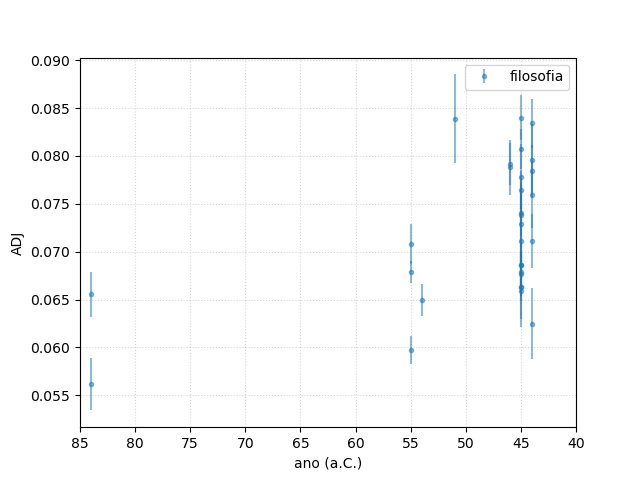
\includegraphics[width=0.5\textwidth]{graficos/ADJ_no_tempo.png} \text{\texttt{ADJ}} \\
		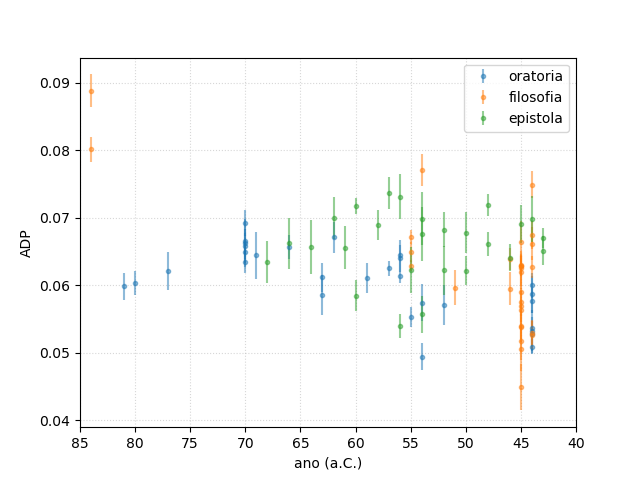
\includegraphics[width=0.5\textwidth]{graficos/ADP_no_tempo.png} \text{\texttt{ADP}} \\
	\end{multicols}\vspace{-0.75cm}
	\begin{multicols}{2}
		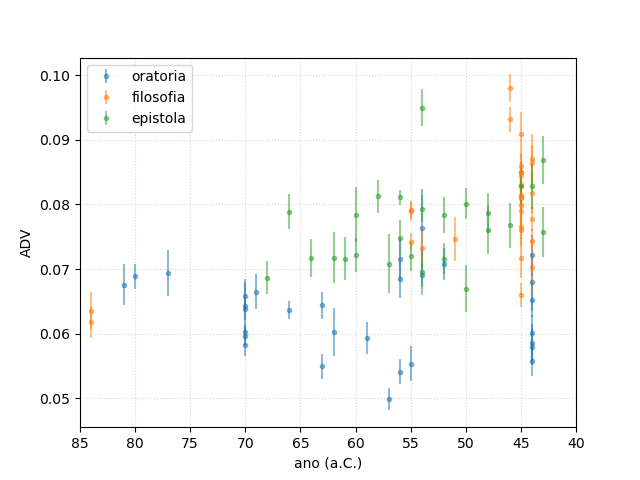
\includegraphics[width=0.5\textwidth]{graficos/ADV_no_tempo.png} \text{\texttt{ADV}} \\
		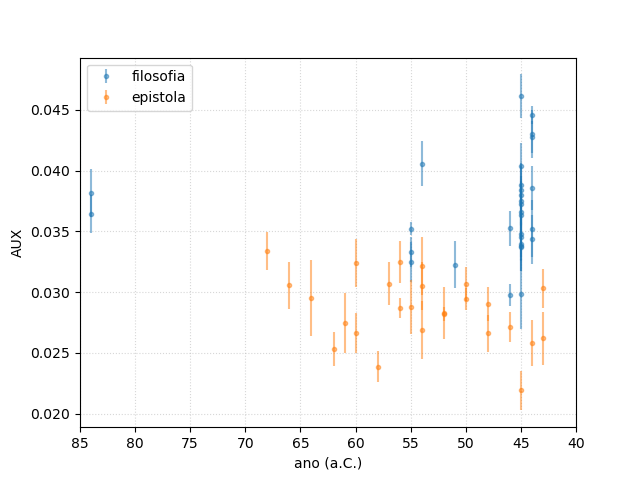
\includegraphics[width=0.5\textwidth]{graficos/AUX_no_tempo.png} \text{\texttt{AUX}} \\
	\end{multicols}\vspace{-0.75cm}
	\begin{multicols}{2}
		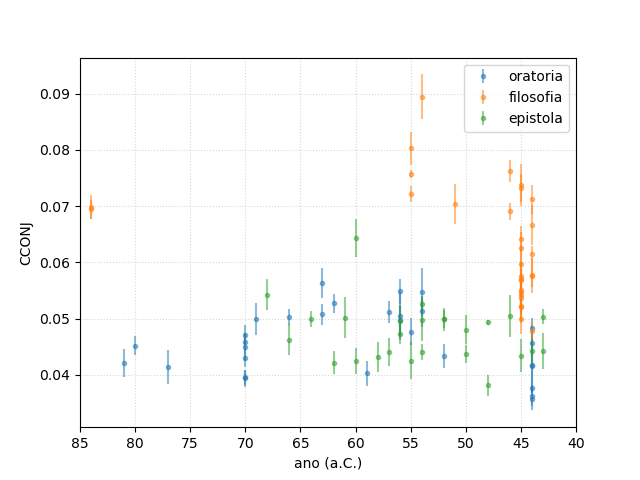
\includegraphics[width=0.5\textwidth]{graficos/CCONJ_no_tempo.png} \text{\texttt{CCONJ}} \\
		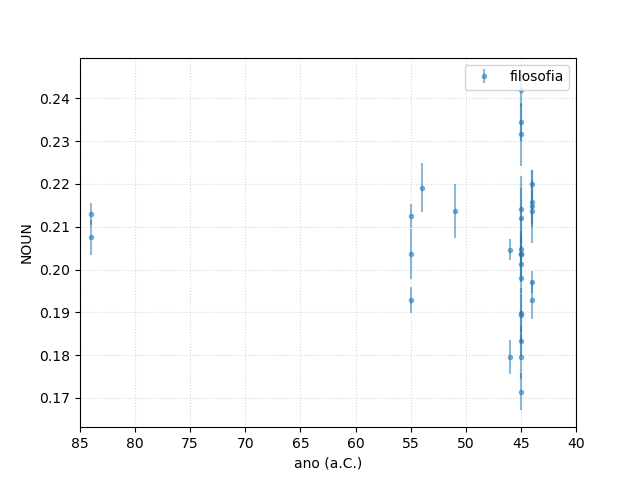
\includegraphics[width=0.5\textwidth]{graficos/NOUN_no_tempo.png} \text{\texttt{NOUN}} \\
	\end{multicols}
	\caption{Evolução no tempo das médias, em cada texto, de densidade das \emph{tags} de POS (ocorrências por \emph{token}). Dados referentes a textos pertencentes aos diversos gêneros em questão aparecem discriminados por cor. Continua.}
	\label{fig:serie1}
\end{figure}
\begin{figure}[htpb!]
	\centering
	\begin{multicols}{2}
		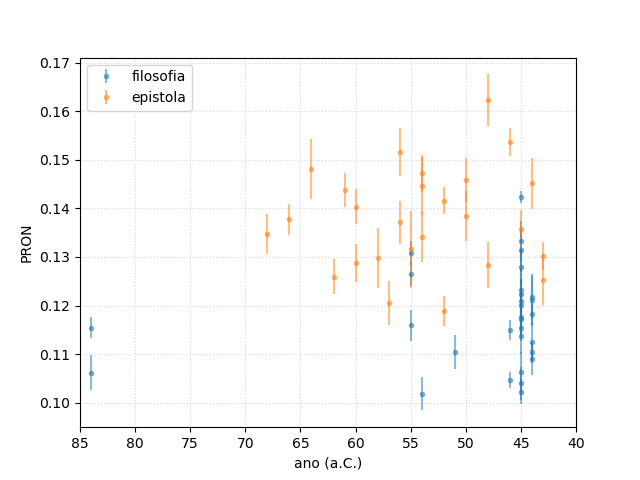
\includegraphics[width=0.5\textwidth]{graficos/PRON_no_tempo.png} \text{\texttt{PRON}} \\ 
		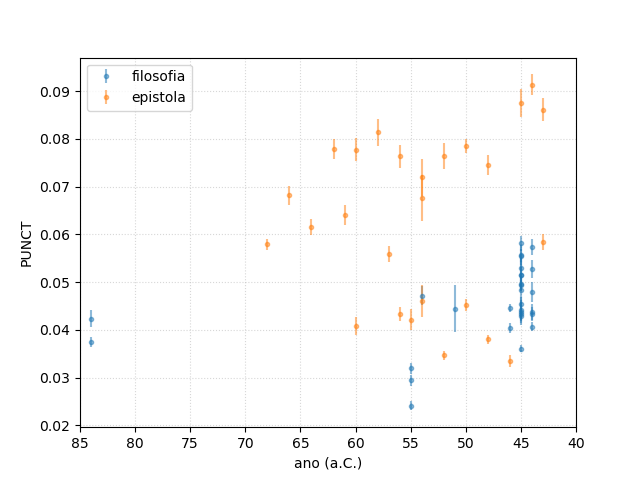
\includegraphics[width=0.5\textwidth]{graficos/PUNCT_no_tempo.png} \text{\texttt{PUNCT}} \\
	\end{multicols}\vspace{-0.75cm}
	\begin{multicols}{2}
		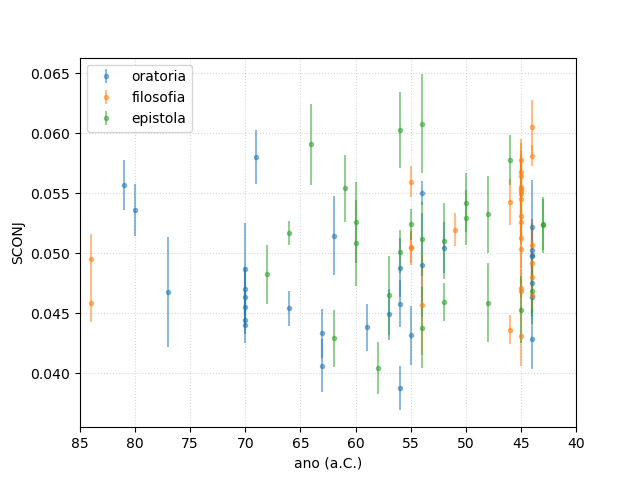
\includegraphics[width=0.5\textwidth]{graficos/SCONJ_no_tempo.png} \text{\texttt{SCONJ}} \\
		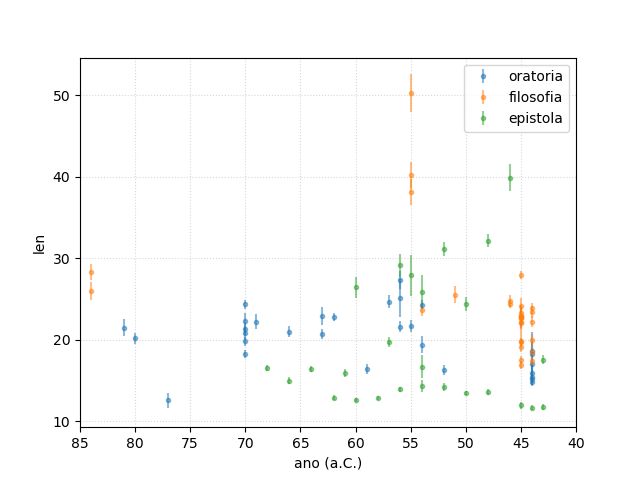
\includegraphics[width=0.5\textwidth]{graficos/len_no_tempo.png} \text{\texttt{Tam}} \\
	\end{multicols}%\vspace{-0.75cm}
	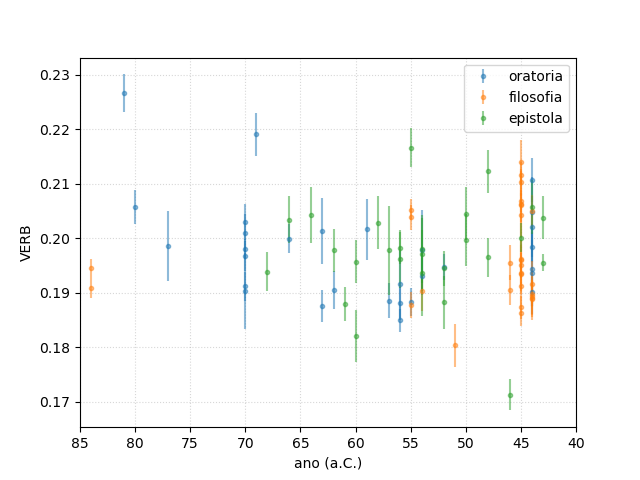
\includegraphics[width=0.5\textwidth]{graficos/VERB_no_tempo.png} \\ \text{\texttt{VERB}} \\ \vspace{0.5cm}
	\caption{Evolução no tempo das médias, em cada texto, de densidade das \emph{tags} de POS (ocorrências por \emph{token}). Dados referentes a textos pertencentes aos diversos gêneros em questão aparecem discriminados por cor. Continuação.}
	\label{fig:serie2}
\end{figure}

Vemos nos gráficos das Figuras \ref{fig:serie1} e \ref{fig:serie2} que não há nenhuma tendência de variação considerável no tempo das variáveis $m^p_i$ que representam as médias de densidade de ocorrência de \emph{tags} de POS; ao contrário, a dispersão desses valores dentro de um mesmo período é claramente dominante sobre variações que possam ocorrer ao longo do tempo.

\subsection{Análise de $\chi^2$}
Exibimos na Figura \ref{fig:histogramas} os dados $m^p_i$ histogramados para cada $p$, agrupados por cor segundo o gênero de $i$:

\begin{figure}[htpb!]
\centering
\begin{multicols}{3}
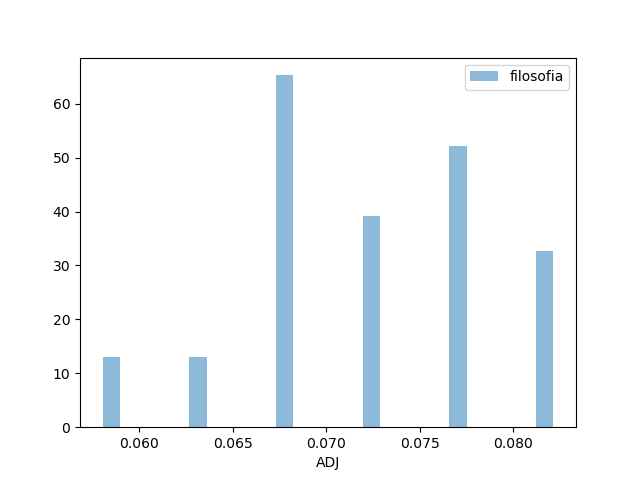
\includegraphics[width=0.33\textwidth]{graficos/histograma_ADJ.png} \text{\texttt{ADJ}} \\
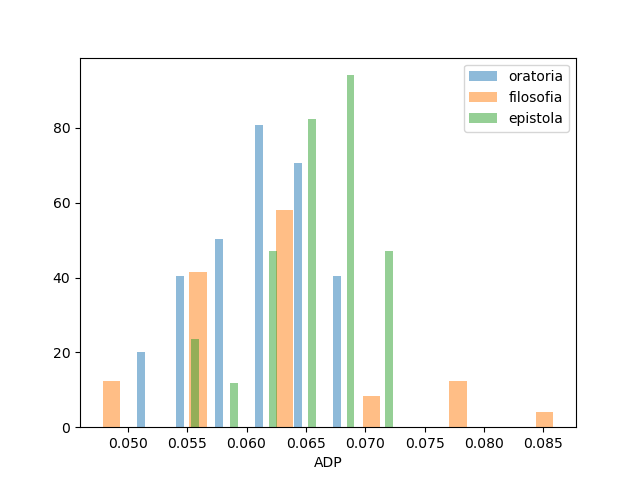
\includegraphics[width=0.33\textwidth]{graficos/histograma_ADP.png} \text{\texttt{ADP}} \\
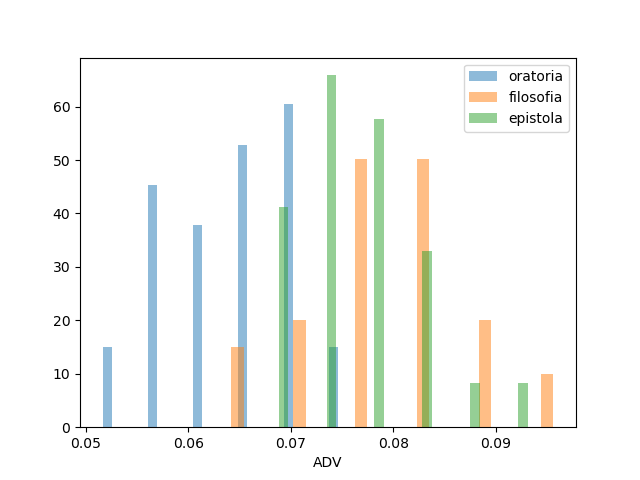
\includegraphics[width=0.33\textwidth]{graficos/histograma_ADV.png} \text{\texttt{ADV}} \\
\end{multicols}
\begin{multicols}{3}
	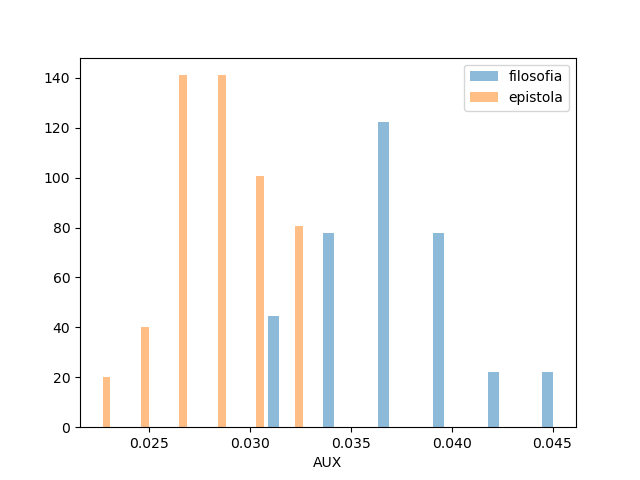
\includegraphics[width=0.33\textwidth]{graficos/histograma_AUX.png} \text{\texttt{AUX}} \\
	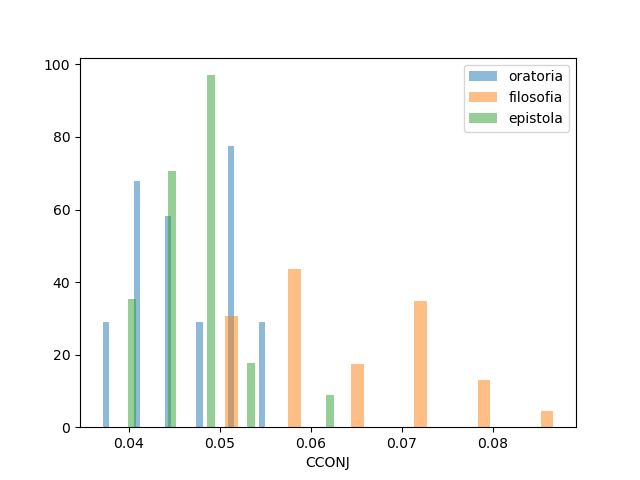
\includegraphics[width=0.33\textwidth]{graficos/histograma_CCONJ.png} \text{\texttt{CCONJ}} \\
	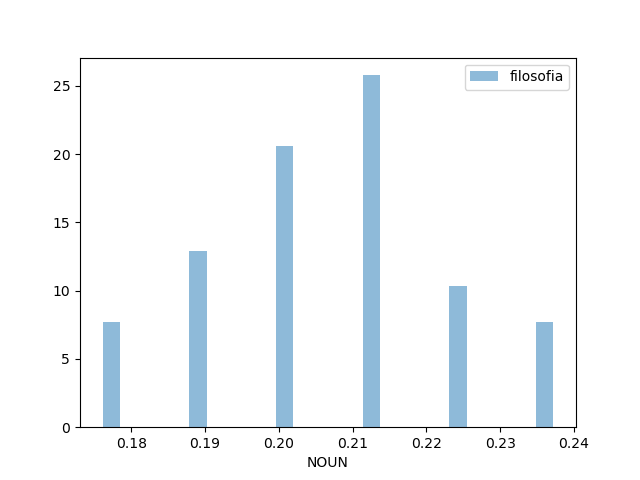
\includegraphics[width=0.33\textwidth]{graficos/histograma_NOUN.png} \text{\texttt{NOUN}} \\
\end{multicols}
\begin{multicols}{3}
	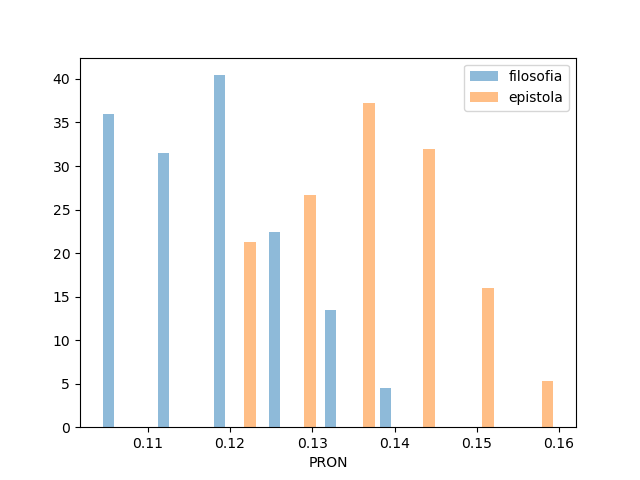
\includegraphics[width=0.33\textwidth]{graficos/histograma_PRON.png} \text{\texttt{PRON}} \\
	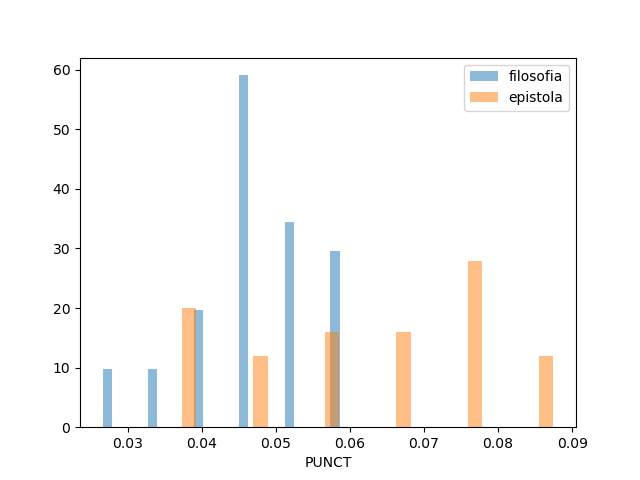
\includegraphics[width=0.33\textwidth]{graficos/histograma_PUNCT.png} \text{\texttt{PUNCT}} \\
	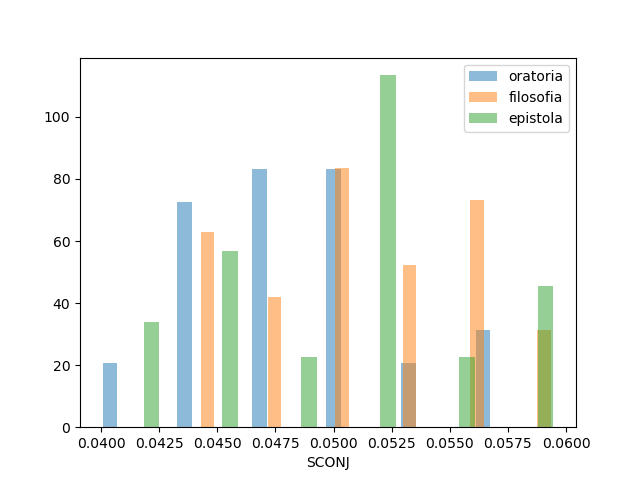
\includegraphics[width=0.33\textwidth]{graficos/histograma_SCONJ.png} \text{\texttt{SCONJ}} \\
	\end{multicols}
\begin{multicols}{2}
	\hspace*{1.75cm}
	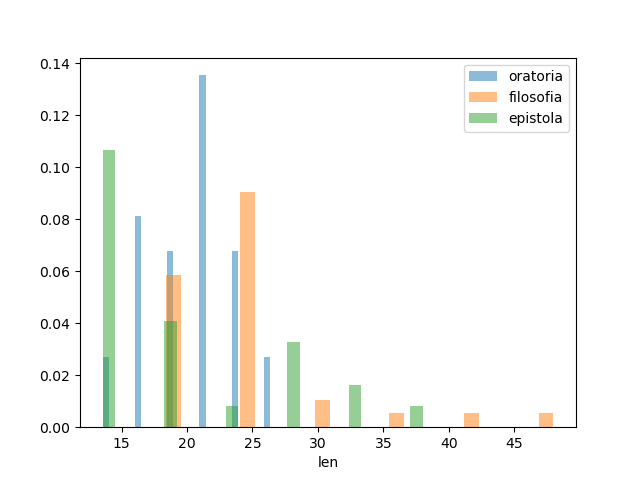
\includegraphics[width=0.33\textwidth]{graficos/histograma_len.png} \\ \hspace*{1.75cm} \text{\texttt{Tam}} \\
	\hspace*{-1.75cm}
	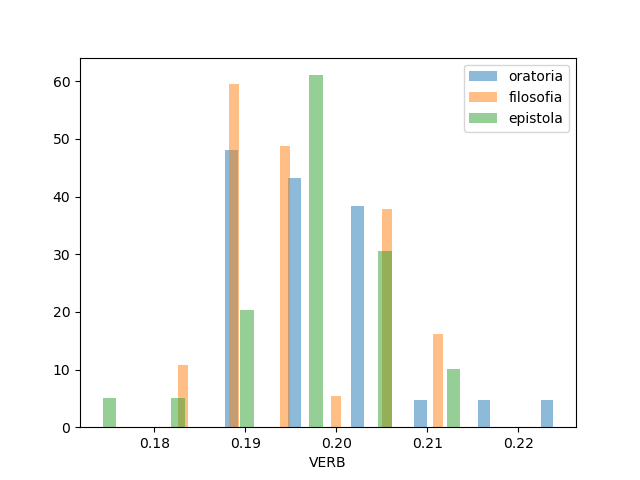
\includegraphics[width=0.33\textwidth]{graficos/histograma_VERB.png} \\ \hspace*{-1.75cm} \text{\texttt{VERB}} \\
\end{multicols}
\caption{Distribuição das densidades de \emph{tags} de POS (ocorrências pro \emph{token}) para cada \emph{tag}. Os dados referentes a textos classificados nos diversos gêneros aparecem discriminados por cor. Nos gráficos somente estão presentes os dados relativos a textos para cujo gênero a \emph{tag} em questão tenha sido selecionada segundo discutido (ver o algoritmo \texttt{tagselect} no Apêndice \ref{ap:tagselect}).}
\label{fig:histogramas}
\end{figure}

\begin{figure}[htpb!]
	\centering
	\begin{multicols}{3}
		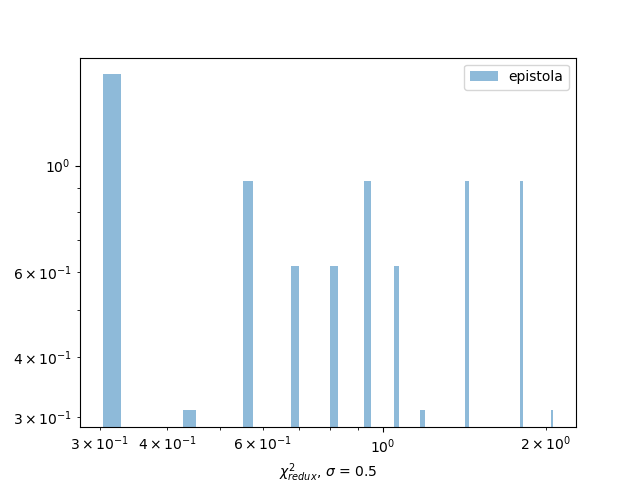
\includegraphics[width=0.33\textwidth]{graficos/histograma1_epistola.png} \\ \vspace{0.15cm} \text{$g =$ \texttt{epistola}} \\
		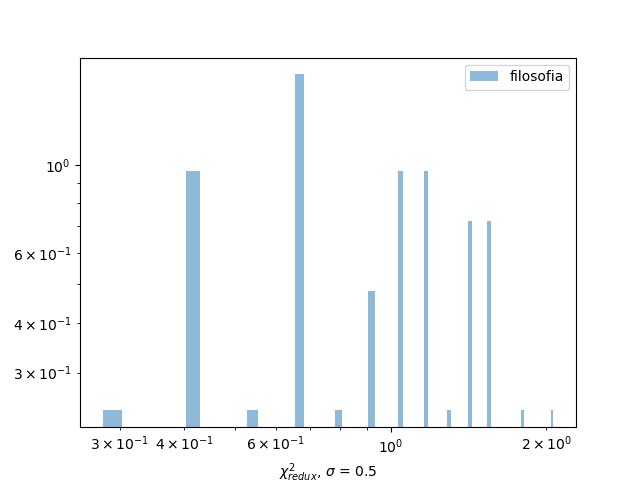
\includegraphics[width=0.33\textwidth]{graficos/histograma1_filosofia.png} \\ \vspace{0.15cm} \text{$g =$ \texttt{filosofia}} \\
		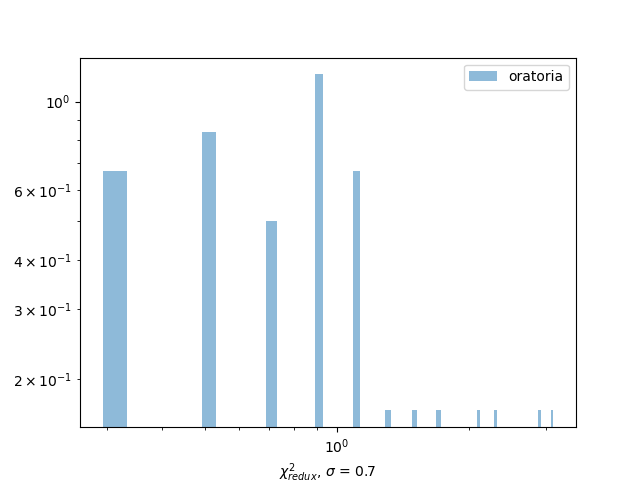
\includegraphics[width=0.33\textwidth]{graficos/histograma1_oratoria.png} \\ \vspace{0.15cm} \text{$g =$ \texttt{oratoria}} \\ 
	\end{multicols}
	\begin{multicols}{3}
		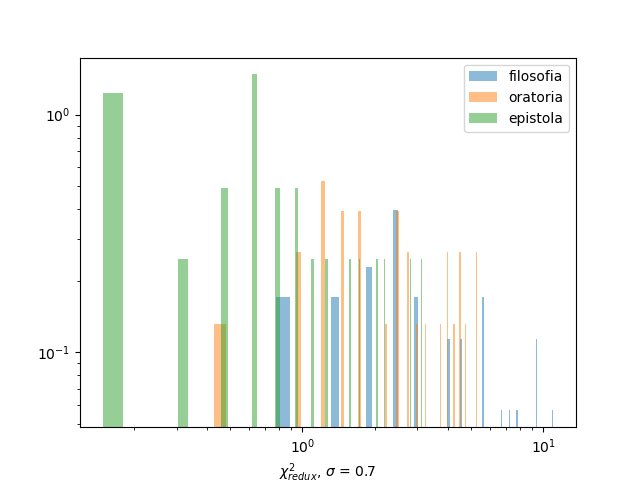
\includegraphics[width=0.33\textwidth]{graficos/histograma3_epistola.png} \\ \vspace{0.15cm} \text{$g =$ \texttt{epistola}} \\
		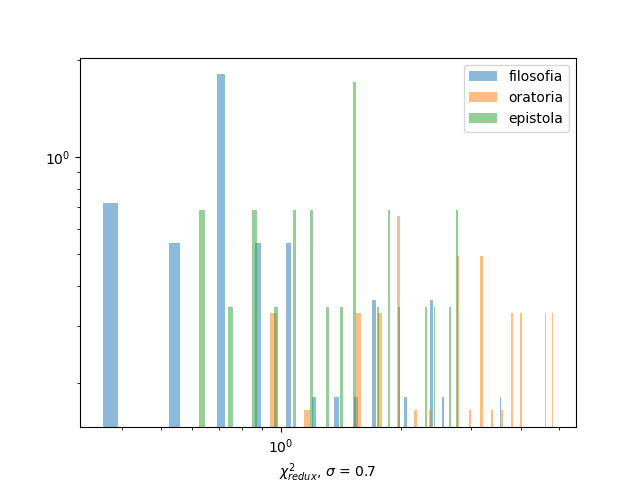
\includegraphics[width=0.33\textwidth]{graficos/histograma3_filosofia.png} \\ \vspace{0.15cm}  \text{$g =$ \texttt{filosofia}} \\
		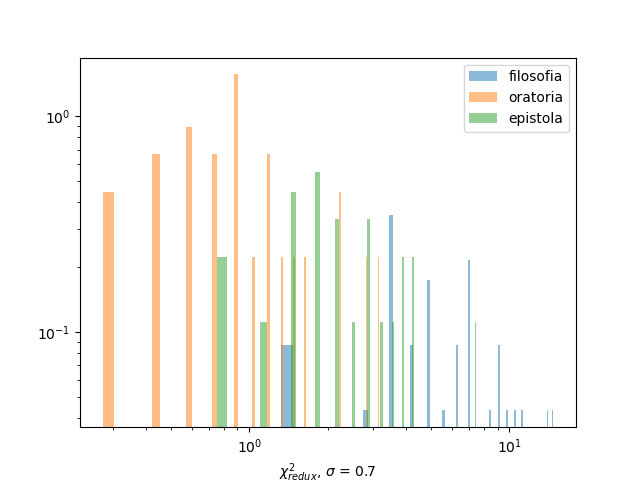
\includegraphics[width=0.33\textwidth]{graficos/histograma3_oratoria.png} \\ \vspace{0.15cm} \text{$g =$ \texttt{oratoria}} \\
	\end{multicols}
	\begin{multicols}{3}
		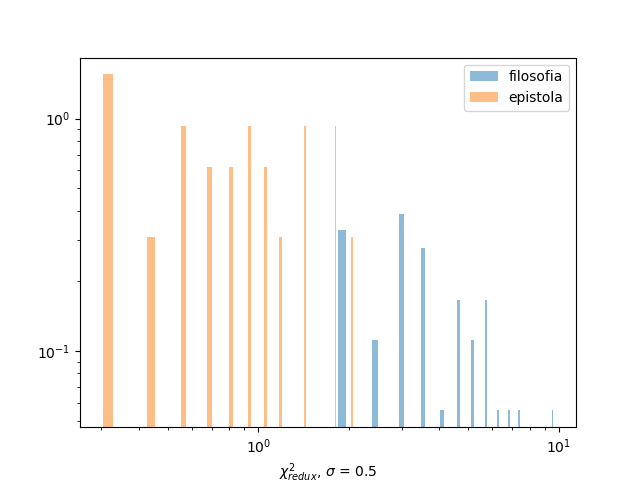
\includegraphics[width=0.33\textwidth]{graficos/histograma2_epistola_filosofia.png} \\ \vspace{0.15cm} \text{$g =$ \texttt{epistola}} \\
		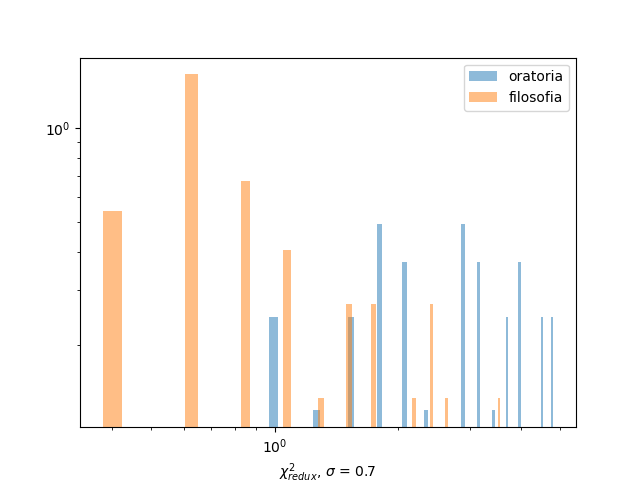
\includegraphics[width=0.33\textwidth]{graficos/histograma2_filosofia_oratoria.png} \\ \vspace{0.15cm} \text{$g =$ \texttt{filosofia}} \\
		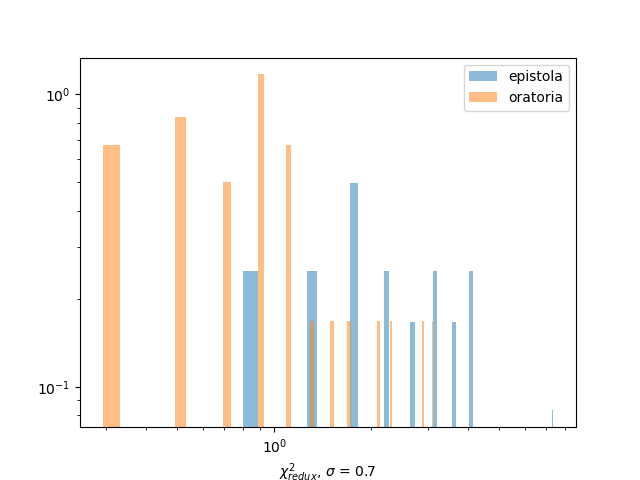
\includegraphics[width=0.33\textwidth]{graficos/histograma2_oratoria_epistola.png} \\ \vspace{0.15cm} \text{$g =$ \texttt{oratoria}} \\
	\end{multicols}
	\begin{multicols}{3}
		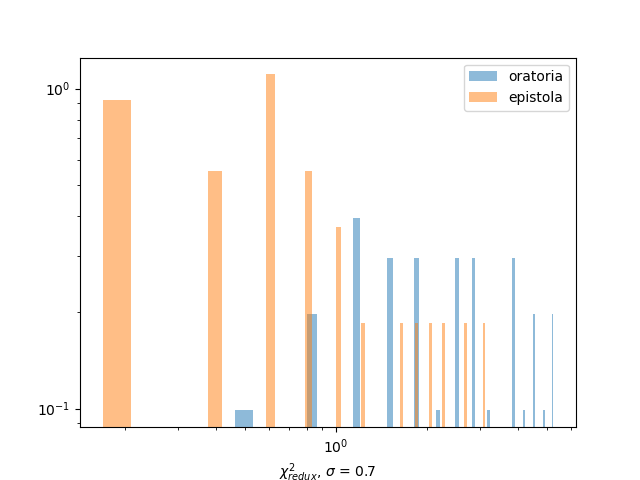
\includegraphics[width=0.33\textwidth]{graficos/histograma2_epistola_oratoria.png} \\ \vspace{0.15cm} \text{$g =$ \texttt{epistola}} \\
		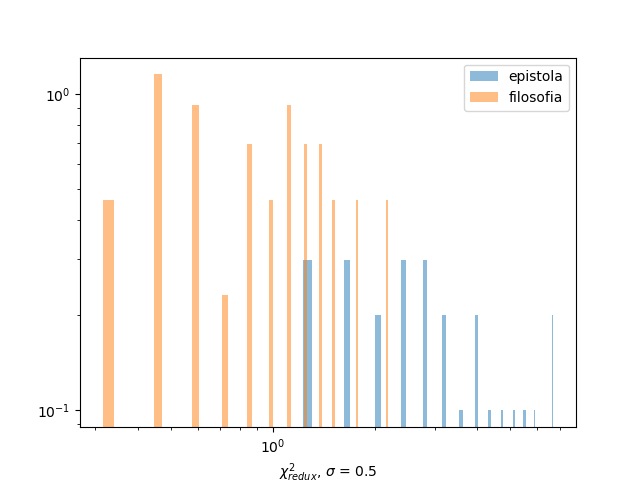
\includegraphics[width=0.33\textwidth]{graficos/histograma2_filosofia_epistola.png} \\ \vspace{0.15cm} \text{$g =$ \texttt{filosofia}} \\
		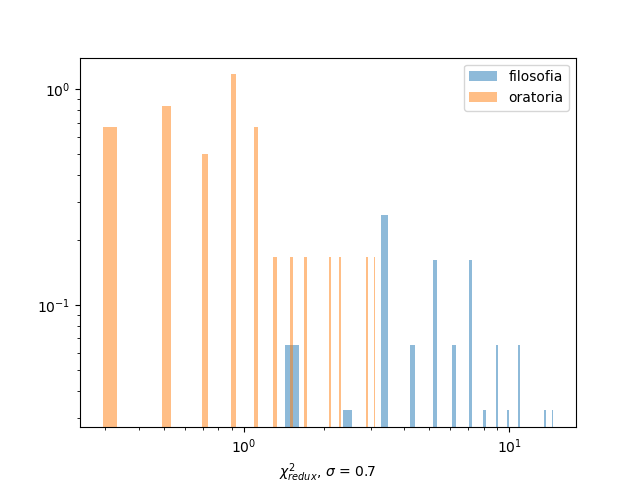
\includegraphics[width=0.33\textwidth]{graficos/histograma2_oratoria_filosofia.png} \\ \vspace{0.15cm} \text{$g =$ \texttt{oratoria}} \\
	\end{multicols}
	\caption{Distribuição dos valores de $\chi^2_g$ reduzido, para os diversos valores de $g$ (gênero). Os dados referentes a textos classificados segundo os distintos gêneros aparecem discriminados por cor. As \emph{tags} de POS utilizadas para o cálculo de $\chi^2_g$ são aquelas selecionadas concomitantemente para os gêneros em análise segundo discutido (ver o algoritmo \texttt{tagselect} no Apêndice \ref{ap:tagselect}), e podem ser identificadas a partir da Figura \ref{fig:histogramas}.}
	\label{fig:histogramas_chis}
\end{figure}

\break

Nota-se que, fixando um gênero $g$, diversas das variáveis $g \ni i \mapsto m^p_i$ aparentam normalidade, embora algumas, sobretudo para $p = $ \texttt{PRON} em $g = $ \texttt{filosofia}, presumivelmente se comportem mais como distribuições de Poisson, as quais, em todo caso, costumam descrever processos de contagens para \underline{poucas} contagens, deixando-se aproximar pela gaussiana conforme a quantidade de contagens aumenta. Quanto às correlações entre as variáveis, ainda que não seja essencial utilizar no cálculo de $\chi^2$ variáveis descorrelacionadas (mas sim independentes!), é importante notar que existe um padrão complexo de correlação entre as diversas variáveis, sugerindo que eles não possam ser bem aproximadas por variáveis aleatórias independentes. Na Figura \ref{fig:dispersoes2}, observamos como a \emph{tag} \texttt{NOUN} aparece fortemente correlacionada com \texttt{PRON} para o gênero \texttt{filosofia}, ao mesmo tempo que aparenta pouca correlação com \texttt{ADJ} (dois últimos gráficos da figura); isso certamente se reflete em correlações entre \texttt{ADJ} e \texttt{PRON} e as demais \emph{tags}. Por exemplo, na mesma figura observamos correlação entre \texttt{PRON} e \texttt{SCONJ} quando tomamos separadamente as distribuições de \texttt{filosofia} e \texttt{oratoria}; por inspeção visual, percebe-se que se as tomássemos conjuntamente, a correlação ficaria bastante atenuada. 

Já na Figura \ref{fig:histogramas_chis}, exibimos as distribuições da função $\chi^2_g$ definida em \eqref{eq:chi_definitivo}, para diversos valores de $g$. As \emph{tags} empregadas no somatório de \eqref{eq:chi_definitivo} são aquelas cujos dados estão disponíveis concomitantemente para \underline{todos} os gêneros em comparação em cada gráfico. Assim, na primeira fileira da figura, os gráficos referem-se às distribuições de $\chi^2_g$ definidos com as \emph{tags} selecionadas por \texttt{tagselect} para \texttt{oratoria}, \texttt{filosofia} e \texttt{epistola}, descritas na Seção \ref{sec:metodologia}; na segunda fileira, os gráficos trazem $\chi^2_g$ em que se utilizam apenas as \emph{tags} na intersecção dos três conjuntos, e nas demais fileiras, \emph{tags} nas intersecção dos conjuntos de \emph{tags} referentes aos dois gêneros em tela. Outras seleções de \emph{tags} seriam possíveis (desde que haja dados disponíveis para cada uma), por exemplo aquelas que, visualmente, nas Figuras \ref{fig:dispersoes1} e \ref{fig:dispersoes2}, mostrem-se mais adequadas para separar dados de um ou outro gênero.

Qualquer que seja o conjunto de \emph{tags} utilizadas no somatório de $\chi^2_g$, os resultados permanecem inalterados do ponto de vista qualitativo: os textos pertencentes ao gênero $g$ sistematicamente apresentam valores de $\chi^2_g$ mais baixos que os demais, a ampla maioria deles dentro de um intervalo de um desvio padrão entorno da média, e o formato das distribuições de $g \ni i \mapsto \chi^2_g(x_i)$ é compatível com o que se esperaria de uma genuína distribuição de $\chi^2$. Para textos que não sejam do gênero $g$, na maioria das vezes os valores de $\chi^2_g$ superam a média por mais que dois ou mesmo três desvios padrões; é o caso dos textos de \texttt{filosofia} quando comparados com $\chi^2_g$ para $g = $ \texttt{epistola}, usando as \emph{tags} desses dois gêneros (primeira coluna, terceira fileira da figura). Contudo, essa é uma conclusão longe de ser geral, por exemplo no cálculo de $\chi^2_g$ em que se utilizam \emph{tags} dos três gêneros, notadamente para $g =$ \texttt{epistola} (primeira coluna, segunda fileira) e para $g = $ \texttt{filosofia}  (segunda coluna, segunda fileira). Assim, demonstra-se a compatibilidade das distribuições $g \ni i \mapsto m^p_i$ enquanto observações de variáveis aleatórias $m_g^p$ distintas para cada gênero e mutuamente independentes (dentro dos conjuntos de \emph{tags} selecionadas por \emph{tagselect}), ainda que para alguns valores de $p$ as médias e variâncias dessas distribuições possam coincidir entre os gêneros, como veremos adiante na Seção \ref{sec:dispersao}.

\subsection{Análise de dispersão}\label{sec:dispersao}
As análises de $\chi^2$ permitiram confirmar que um mesmo autor produz distribuições de densidade de POS diferentes segundo escreve em diversos gêneros; entretanto, também evidenciou a dificuldade de separar textos por gênero com base apenas nos valores de $\chi^2$, algo que havíamos feito para atribuir autoria, no EP 7. Isso se deve ao fato de as diferenças de densidade média entre um gênero e outro serem, via de regra, ordens de grandeza menores que seus respectivos desvios padrões. Entretanto, com uma análise mais fina é possível identificar características que classificam os textos como pertencentes a um ou outro gênero. Em muitos dos gráficos de dispersão das Figuras \ref{fig:dispersoes1} e \ref{fig:dispersoes2} vemos claramente como \texttt{epistola} e \texttt{filosofia} ocupam regiões distintas do espaço $p_x \times p_y$; na dispersão \texttt{PRON} $\times$ \texttt{AUX} pode-se mesmo separar esses gêneros por um classificador linear! A identificação do gênero \texttt{oratoria} parece menos clara, pois em muitos casos sobrepõe-se com \texttt{epistola}\footnote{Talvez porque em suas correspondências Cícero não deixa de discursar de maneira retoricamente conformada, ainda que no âmbito privado, enquanto que na obra filosófica haja uma preponderância de diálogos em que as falas têm mais traços de oralidade e espontaneidade?}, ainda assim não impossível, considerando \texttt{ADV} $\times$ \texttt{ADP}, em que parece se separar dos demais, ou diversos outros, como \texttt{CCONJ} $\times$ \texttt{SCONJ}, em que se separa bem de \texttt{filosofia}.

É importante lembrar que a comparação de dispersão por duplas de \emph{tags} dá-se apenas por motivos de visualização gráfica; eventualmente, se comparássemos três ou mais \emph{tags} poderíamos determinar de maneira mais precisa características não óbvias dos textos, envolvendo diversas relações entre as médias de densidade de POS, que os classificariam segundo gênero. Tal estudo poderia ser realizado por meio da estruturação de redes neurais que utilizem que utilizem como \emph{embedding} para os textos a classificar os valores de $m_i^p$ para as \emph{tags} $p$ disponíveis. 

\begin{figure}[htpb!]
	\centering
	\begin{multicols}{3}
		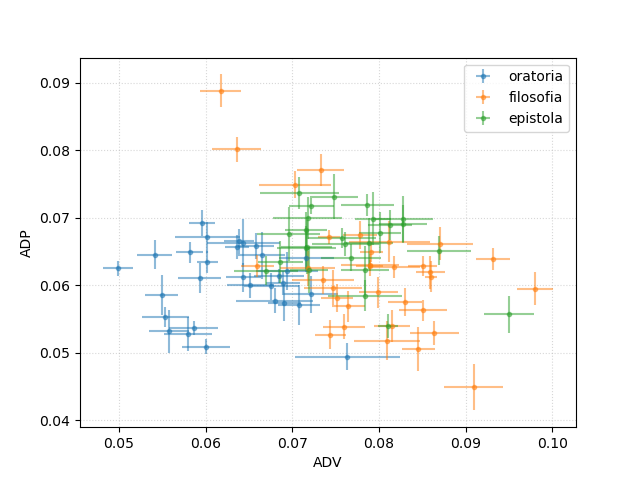
\includegraphics[width=0.33\textwidth]{graficos/ADP_x_ADV.png} \text{\texttt{ADV} $\times$ \texttt{ADP}} \\
		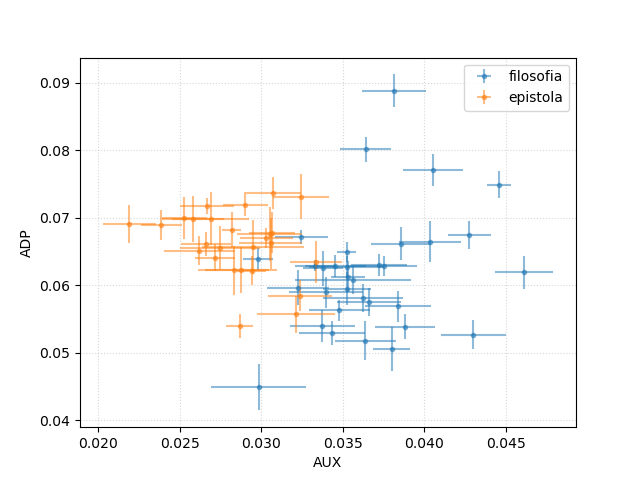
\includegraphics[width=0.33\textwidth]{graficos/ADP_x_AUX.png} \text{\texttt{AUX} $\times$ \texttt{ADP}} \\
		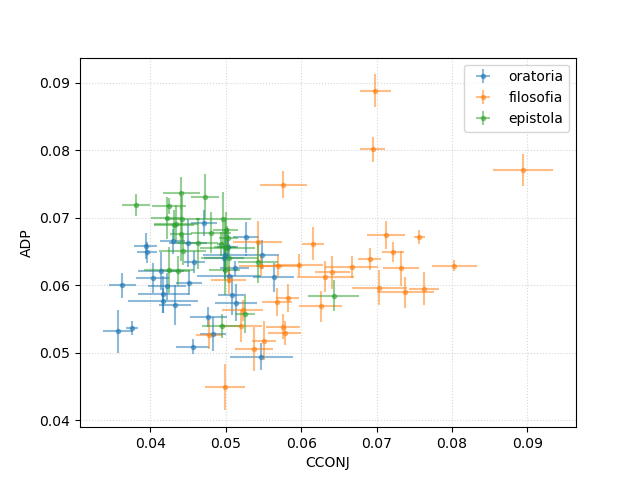
\includegraphics[width=0.33\textwidth]{graficos/ADP_x_CCONJ.png} \text{\texttt{CCONJ} $\times$ \texttt{ADP}} \\
	\end{multicols}\vspace{-0.8cm}
	\begin{multicols}{3}
		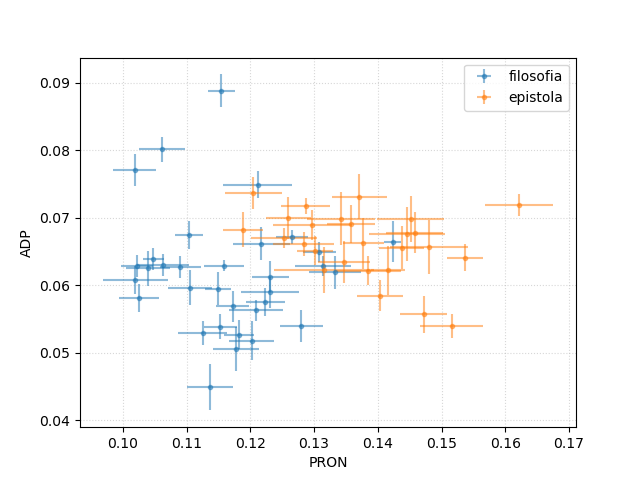
\includegraphics[width=0.33\textwidth]{graficos/ADP_x_PRON.png} \text{\texttt{PRON} $\times$ \texttt{ADP}} \\
		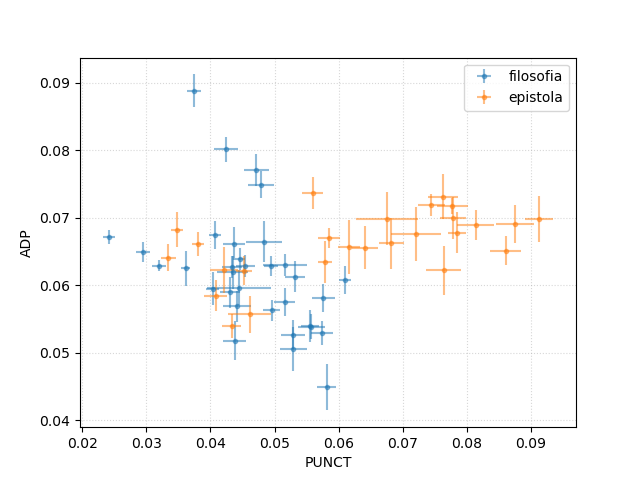
\includegraphics[width=0.33\textwidth]{graficos/ADP_x_PUNCT.png} \text{\texttt{PUNCT} $\times$ \texttt{ADP}} \\
		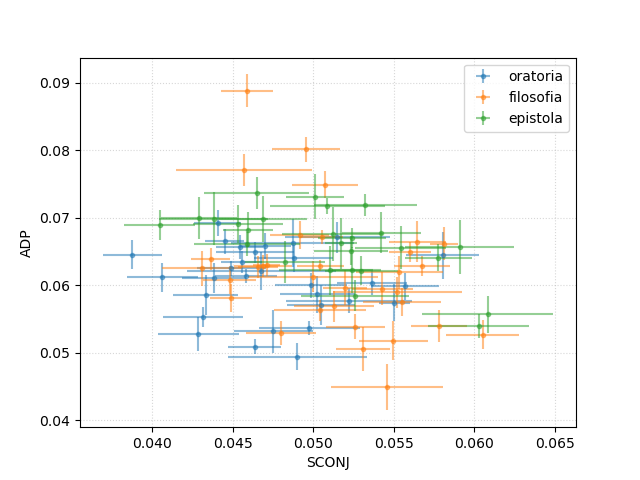
\includegraphics[width=0.33\textwidth]{graficos/ADP_x_SCONJ.png} \text{\texttt{SCONJ} $\times$ \texttt{ADP}} \\
	\end{multicols}\vspace{-0.8cm}
	\begin{multicols}{3}
		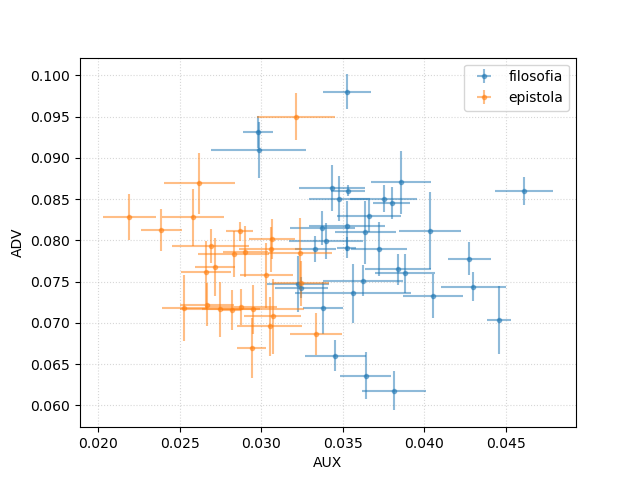
\includegraphics[width=0.33\textwidth]{graficos/ADV_x_AUX.png} \text{\texttt{AUX} $\times$ \texttt{ADV}} \\
		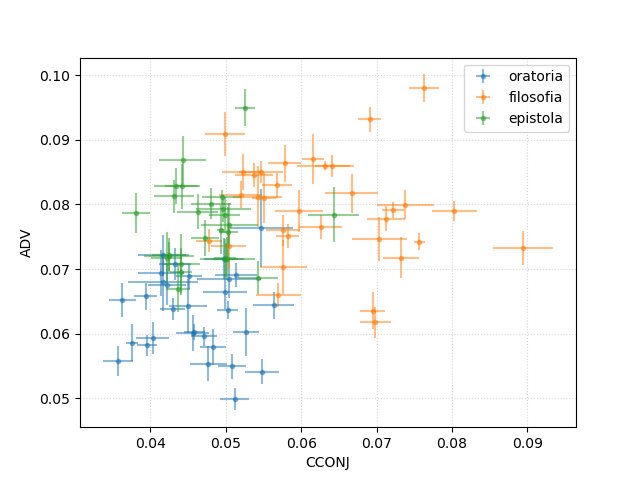
\includegraphics[width=0.33\textwidth]{graficos/ADV_x_CCONJ.png} \text{\texttt{CCONJ} $\times$ \texttt{ADV}} \\
		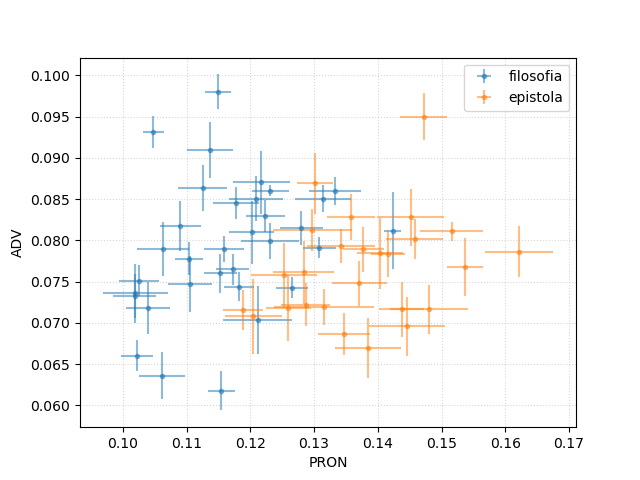
\includegraphics[width=0.33\textwidth]{graficos/ADV_x_PRON.png} \text{\texttt{PRON} $\times$ \texttt{ADV}} \\
	\end{multicols}\vspace{-0.8cm}
	\begin{multicols}{3}
		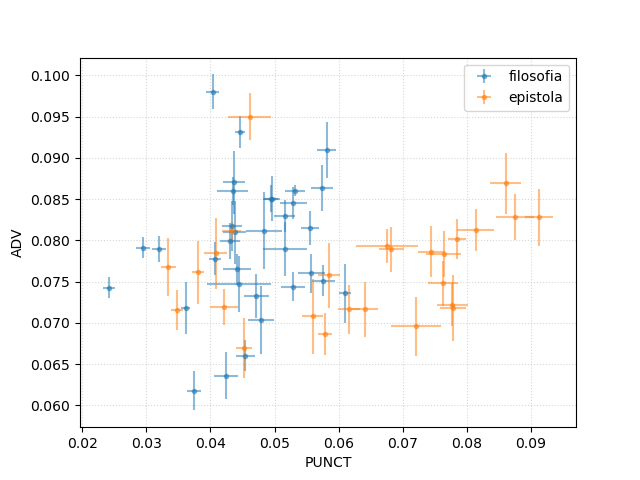
\includegraphics[width=0.33\textwidth]{graficos/ADV_x_PUNCT.png} \\ \text{\texttt{PUNCT} $\times$ \texttt{ADV}} \\
		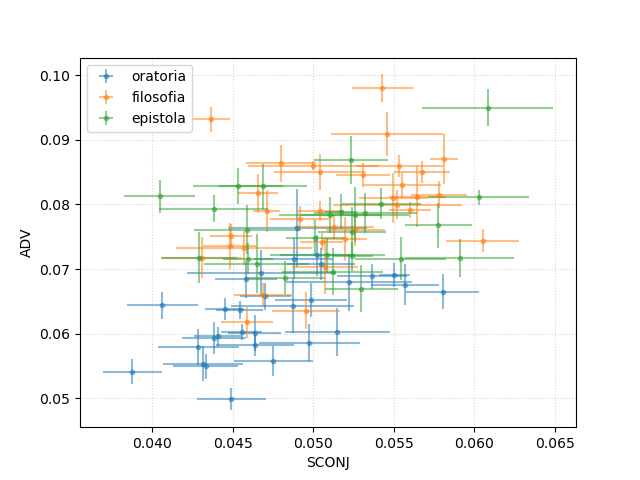
\includegraphics[width=0.33\textwidth]{graficos/ADV_x_SCONJ.png} \\ \text{\texttt{SCONJ} $\times$ \texttt{ADV}} \\
		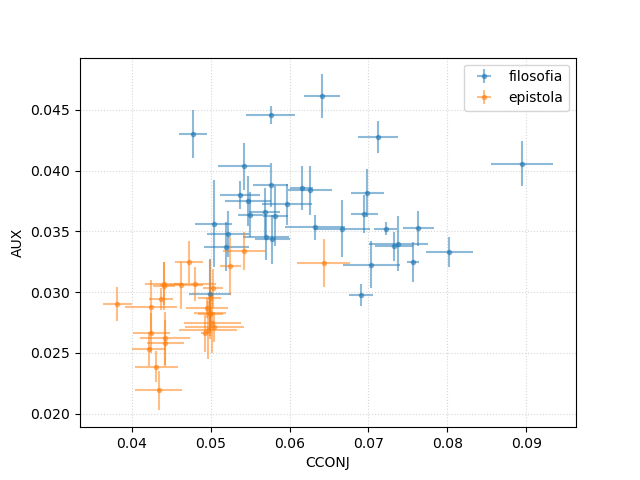
\includegraphics[width=0.33\textwidth]{graficos/AUX_x_CCONJ.png} \\ \text{\texttt{CCONJ} $\times$ \texttt{AUX}} \\
	\end{multicols}\vspace{-0.8cm}
	\begin{multicols}{3}
		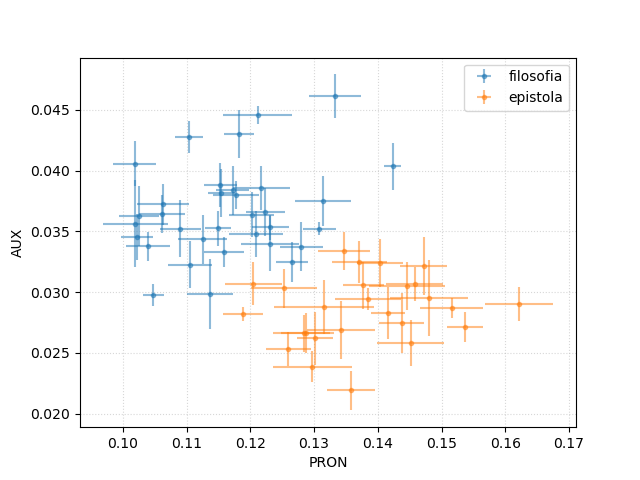
\includegraphics[width=0.33\textwidth]{graficos/AUX_x_PRON.png} \\ \text{\texttt{PRON} $\times$ \texttt{AUX}} \\
		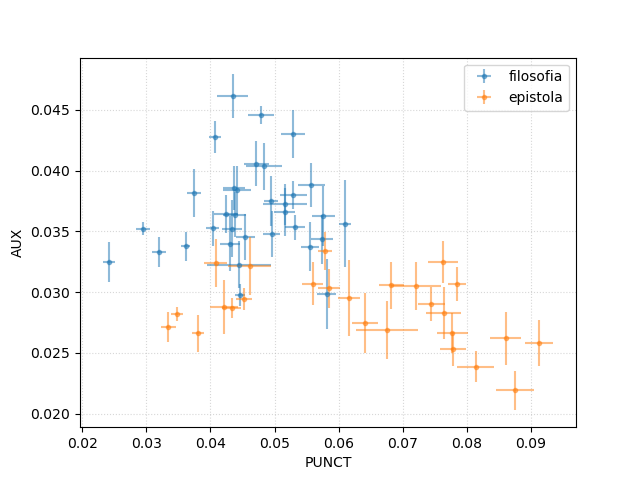
\includegraphics[width=0.33\textwidth]{graficos/AUX_x_PUNCT.png} \\ \text{\texttt{PUNCT} $\times$ \texttt{AUX}} \\
		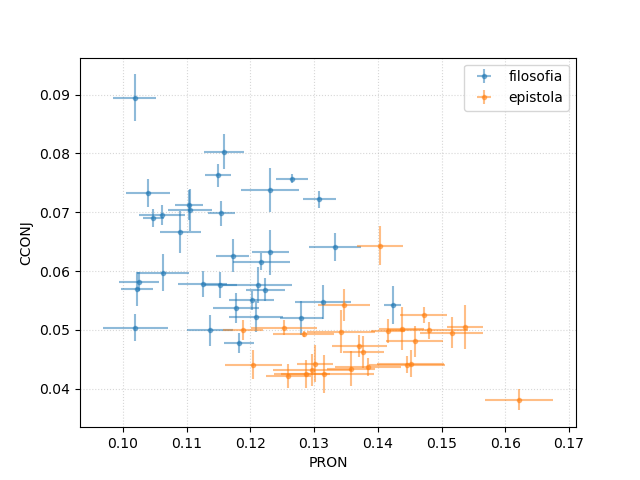
\includegraphics[width=0.33\textwidth]{graficos/CCONJ_x_PRON.png} \\ \text{\texttt{PRON} $\times$ \texttt{CCONJ}} \\
	\end{multicols}\vspace{-0.5cm}
	\caption{Gráficos de dispersão para pares de médias de densidades de \emph{tags} de POS (ocorrências por \emph{token}), discriminados por gênero. Continua.}
	\label{fig:dispersoes1}
\end{figure}

\begin{figure}[htpb!]
	\centering
	\begin{multicols}{3}
		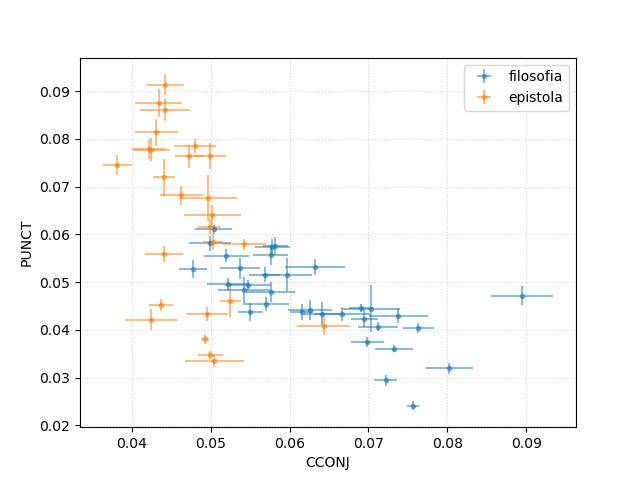
\includegraphics[width=0.33\textwidth]{graficos/PUNCT_x_CCONJ.png} \text{\texttt{CCONJ} $\times$ \texttt{PUNCT}} \\
		\includegraphics[width=0.33\textwidth]{graficos/PUNCT_x_PRON.png} \text{\texttt{PRON} $\times$ \texttt{PUNCT}} \\
		\includegraphics[width=0.33\textwidth]{graficos/SCONJ_x_AUX.png} \text{\texttt{AUX} $\times$ \texttt{SCONJ}} \\
	\end{multicols}\vspace{-0.8cm}
	\begin{multicols}{3}
		\includegraphics[width=0.33\textwidth]{graficos/SCONJ_x_CCONJ.png} \text{\texttt{CCONJ} $\times$ \texttt{SCONJ}} \\
		\includegraphics[width=0.33\textwidth]{graficos/SCONJ_x_PRON.png} \text{\texttt{PRON} $\times$ \texttt{SCONJ}} \\
		\includegraphics[width=0.33\textwidth]{graficos/SCONJ_x_PUNCT.png} \text{\texttt{PUNCT} $\times$ \texttt{SCONJ}} \\
	\end{multicols}\vspace{-0.8cm}
	\begin{multicols}{3}
		\includegraphics[width=0.33\textwidth]{graficos/VERB_x_ADP.png} \text{\texttt{ADP} $\times$ \texttt{VERB}} \\
		\includegraphics[width=0.33\textwidth]{graficos/VERB_x_ADV.png} \text{\texttt{ADV} $\times$ \texttt{VERB}} \\
		\includegraphics[width=0.33\textwidth]{graficos/VERB_x_AUX.png} \text{\texttt{AUX} $\times$ \texttt{VERB}} \\
	\end{multicols}\vspace{-0.8cm}
	\begin{multicols}{3}
		\includegraphics[width=0.33\textwidth]{graficos/VERB_x_CCONJ.png} \\ \text{\texttt{CCONJ} $\times$ \texttt{VERB}} \\
		\includegraphics[width=0.33\textwidth]{graficos/VERB_x_PRON.png} \\ \text{\texttt{PRON} $\times$ \texttt{VERB}} \\
		\includegraphics[width=0.33\textwidth]{graficos/VERB_x_PUNCT.png} \\ \text{\texttt{PUNCT} $\times$ \texttt{VERB}} \\
	\end{multicols}\vspace{-0.8cm}
	\begin{multicols}{3}
		\includegraphics[width=0.33\textwidth]{graficos/VERB_x_SCONJ.png} \\ \text{\texttt{SCONJ} $\times$ \texttt{VERB}} \\
		\includegraphics[width=0.33\textwidth]{graficos/NOUN_x_PRON.png} \\ \text{\texttt{PRON} $\times$ \texttt{NOUN}} \\
		\includegraphics[width=0.33\textwidth]{graficos/ADJ_x_NOUN.png} \\ \text{\texttt{NOUN} $\times$ \texttt{ADJ}} \\
	\end{multicols}\vspace{-0.5cm}
	\caption{Gráficos de dispersão para pares de médias de densidades de \emph{tags} de POS (ocorrências por \emph{token}), discriminados por gênero. Continuação.}
	\label{fig:dispersoes2}
\end{figure}

\section{Conclusão}
As densidades médias de \emph{tags} de POS, em Cícero, variam apreciavelmente, mas sem relação direta com o tempo, podendo em um mesmo ano apresentar variações muito maiores que em décadas. Além disso, constatamos que, para certas \emph{tags}, essas médias distribuem-se normalmente de formas próprias a cada gênero e independentes entre si. Apesar disso, não é possível utilizá-las em testes de $\chi^2$ a fim de classificar os textos de Cícero em gênero, embora elas sejam uma forma de \emph{embedding} que se demonstra promissor para a estruturação de redes neurais que façam tal classificação.

\appendix
\newpage
\section{Código \textsc{Python}}\label{ap:python}
\noindent
Todos os códigos abaixo (e ainda outros, assim como gráficos e diversos dados, brutos e processados), encontram-se disponíveis em \texttt{https://github.com/vbchabu/fll5133\_trabalho\_final} até 31/01/2022.

\subsection{\texttt{amostras.py}}
\noindent
Define a classe \texttt{Amostra} com atributos relativos a textos em análise e métodos para gravação e leitura desses dados em arquivo, já fazendo a análise de \texttt{POS}.
\lstinputlisting[language=Python]{amostras.py}
\

\subsection{\texttt{processo\_nlp.py}}
\noindent
\emph{Script} que efetivamente processa os \emph{corpora} fornecidos e salva os dados para posterior análise.
\lstinputlisting[language=Python]{processo_nlp.py}
\

\subsection{\texttt{tagstats.py}}\label{ap:tagstats}
\noindent
Processa dados linguísticos oriundos de amostras da classe \texttt{Amostra} segundo a metodologia descrita, e salva as diversas estatísticas obtidas em arquivos \texttt{csv}.
\lstinputlisting[language=Python]{tagstats.py}
\

\break

\subsection{\texttt{tagselect.py}}\label{ap:tagselect}
\noindent
Seleciona as \emph{tags} de POS a serem utilizadas em análises de $\chi^2$ a partir de critérios definidos.
\lstinputlisting[language=Python]{tagselect.py}
\

\break

\subsection{\texttt{chi\_quadrado.py}}
\noindent
Calcula as estatísticas referentes às distribuições de distribuições para cada gênero, e define um método para calcular o $\chi^2$ de um texto (com dados fornecidos como \emph{output} de \texttt{tagstats}) com respeito a um gênero.
\lstinputlisting[language=Python]{chi_quadrado.py}
\

%\subsection{\texttt{tagsbank.py}}
%\noindent
%Banco contendo a totalidade das \emph{tags} de POS e DET obtidas na execução de \texttt{processo\_nlp}.
%\lstinputlisting[language=Python]{tagsbank.py}
\end{document}